\documentclass[10pt]{article}

\usepackage{tikz}
\usepackage{pgfplots}
\pgfplotsset{compat=1.17}
\usepackage{amssymb}
\usepackage{amsmath}
\usepackage{mathtools}
\usepackage{indentfirst}
\usepackage{footnote}
\makesavenoteenv{tabular}
\makesavenoteenv{table}
\usepackage[hidelinks]{hyperref}
\usepackage[nameinlink,noabbrev]{cleveref}
\usepackage{multirow}
\usepackage{makecell}
\usepackage[stype=amc,natbib=true,backend=biber,maxbibnames=20]{biblatex}
\bibliography{bibliography}
\usepackage{csagh}
\usepackage{lscape}

\usetikzlibrary{arrows,decorations.markings}

\makeatletter
\DeclareRobustCommand\bigop[2][1]{%
  \mathop{\vphantom{\sum}\mathpalette\bigop@{{#1}{#2}}}\slimits@
}
\newcommand{\bigop@}[2]{\bigop@@#1#2}
\newcommand{\bigop@@}[3]{%
  \vcenter{%
    \sbox\z@{$#1\sum$}%
    \hbox{\resizebox{\ifx#1\displaystyle#2\fi\dimexpr\ht\z@+\dp\z@}{!}{$\m@th#3$}}%
  }%
}
\makeatother


\newcommand{\XORsum}{\DOTSB\bigop[0.92]{\Xi}}
\newcommand{\ANDsum}{\DOTSB\bigop[0.92]{\Lambda}}

% Tikz node styles
\tikzstyle{basic} = [rectangle, minimum width=3cm, minimum height=0.75cm, text width=2.8cm, text centered, draw=black]
\tikzstyle{function} = [rectangle, minimum width=3cm, minimum height=0.75cm,text centered, text width=2.8cm, draw=black, fill=orange!30]
\tikzstyle{ios} = [rectangle, minimum width=3cm, minimum height=0.75cm, text width=2.8cm, text centered, draw=black, fill=green!30]
\tikzstyle{ioe} = [rectangle, minimum width=3cm, minimum height=0.75cm, text width=2.8cm, text centered, draw=black, fill=red!30]

\begin{document}
\begin{opening}

\title{File compression using successive single key bit-shifted XOR functions}

\author{Rosie Bartlett}

\begin{abstract}
Lossless compression is exceptionally useful for data storage on small and large scales. In this paper, I would like to propose a new method for lossless data compression using single key bit shifting and successive XOR functions. This paper is primarily a proof of concept paper to demonstrate the capabilities of this method, which would undoubtedly improve with further research.

\end{abstract}

\keywords{compression, bit shifting, single key, XOR}

\end{opening}


\section{Introduction}\label{sec:intro}

Throughout this paper I will be exploring a new compression method, named SBX(successive bit-shifted XOR) with the file extension \texttt{.sqzr}. SBX takes in a batch of binary strings, and returns a master binary string, set of keys, and set of bit shift lists. SBX is based upon the concept that the master binary string is a general overview of all given binary strings. This overview is then “corrected" by long keys to make the master binary string into the relative binary string for that long key. This long key can be represented as a shorter key, $k_n$ and list of bit shifts, $s_n$, which is how SBX achieves compression.

One key part of SBX is bit shift lists. A bit shift list (BSL) is simply a list of integer values that is used along with a key to represent a long key. Each item in the list is referred to using the notation $s_{n,i}$ for the $i$\textsuperscript{th} value in the bit shift list associated with file $n$. Please note that the term file and binary string will be used interchangeably throughout since they are considered the same within this scope.

Something to sum up the results section and show off how good it is.

\begin{table}[ht]
    \centering
    \begin{tabular}{c >{\raggedleft\arraybackslash}p{5.5cm} >{\raggedleft\arraybackslash}p{3cm}}
        \hline
        Symbol & Description & Type \\
        \Xhline{3\arrayrulewidth}
        $s_n$ & Bit shift list for file $n$ & List of integers \\
        $k_n$ & The associated key for file $n$ & Bit string \\
        $D(k_n,s_n)$ & Decoding function. See \cref{eqn:decodeFunc} & Function \\
        $\XORsum$ & Bitwise XOR shorthand. See \cref{eqn:xorsum} & Operation \\
        $<<$ & Bit shift left & Operation \\
        $I_n$ & Intermediate key, or long key. See \cref{eqn:intermediate} & Bit string \\
        $F_n$ & File $n$, where n$\neq0$ & Bit string \\
        $F_{0C}$ & Calculated $F_0$ for a given key and BSL pairing. This may be an incorrect $F_0$ & Bit
        string \\
        $F_0$ & Compressed file & Bit string \\
        $L(s)$ & Number of items in all bit shift strings & Integer\\
        \hline
    \end{tabular}
    \caption{Notation used throughout this paper, in order of occurrence}
    \label{tab:notationTable}
\end{table}


\section{Method}

SBX compresses files by using a single master file and compressed keys. The compressed keys is how SBX reduces the volume of data stored. An example of this key compression is shown in \cref{subsubsec:example}. Key compression uses shorter keys and BSLs to represent longer keys, shown in \cref{eqn:decodeFunc}.

Since this method involves multiple XOR functions, a shorthand function for recurrent XOR functions has been defined in \cref{eqn:xorsum}.

\begin{equation}\label{eqn:decodeFunc}
    D(k_n,s_n)=\XORsum_{i=1}(k_n << s_{n,i})
\end{equation}
\begin{equation}\label{eqn:xorsum}
    \XORsum_{i=1}^m(x_i)=x_1\oplus x_2\oplus \dots \oplus x_m
\end{equation}
\begin{equation}\label{eqn:intermediate}
    I_n=F_n\oplus F_{0C}
\end{equation}
\begin{equation}
    \ANDsum_{i=1}^m(x_i)=x_0\wedge x_1\wedge \dots \wedge x_m
\end{equation}
\begin{equation}
    S(F)=\ANDsum_{i=1}^n(F_i) \oplus \ANDsum_{i=1}^n(\overline{F_n})
\end{equation}

\subsection{Compression}\label{subsec:compression}

\begin{figure}[h!]
    \centering
    \scalebox{0.9}{
    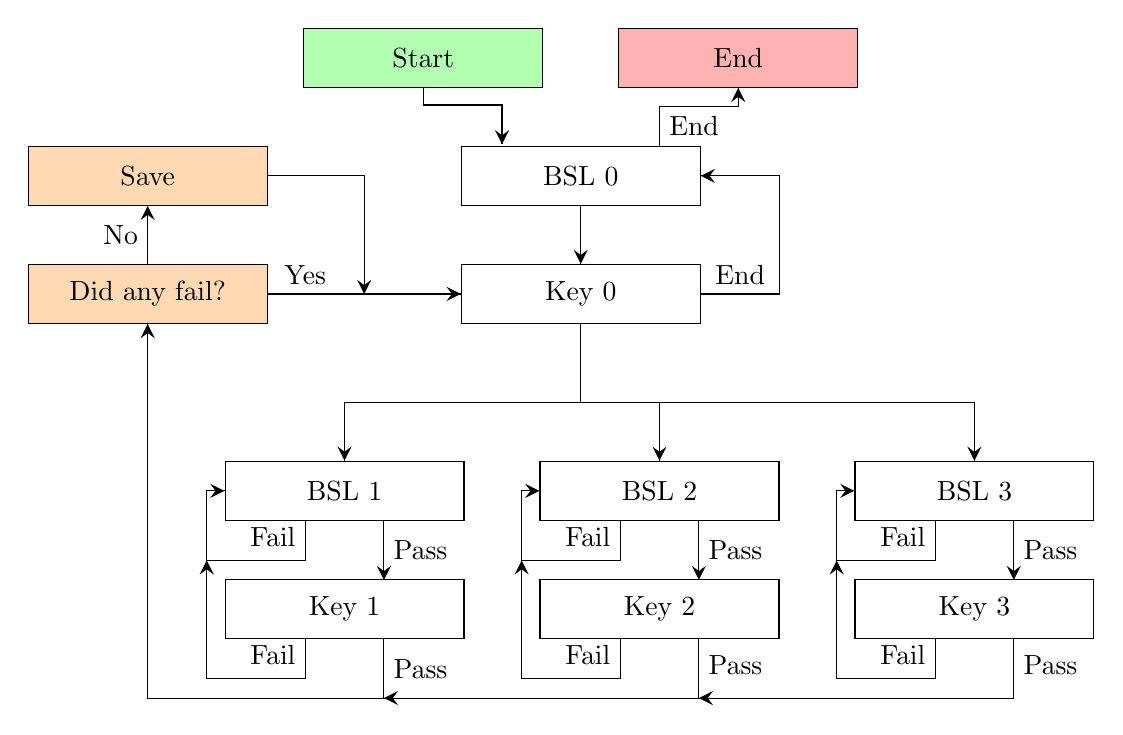
\begin{tikzpicture}[node distance=1.5cm]
    \tikzset{myptr/.style={decoration={markings,mark=at position 1 with %
    {\arrow[scale=1.6,>=stealth]{>}}},postaction={decorate}}}
\node (BSL0) [basic] {BSL 0};
\node (start) [ios, above of=BSL0, xshift=-2cm] {Start};
\node (end) [ioe, above of=BSL0, xshift=2cm] {End};
\node (K0) [basic, below of=BSL0] {Key 0};
\node (FailCheck) [function, left of=K0, xshift=-4cm] {Did any fail?};
\node (Save) [function, above of=FailCheck] {Save};

\node (BSL1) [basic, below of=K0, xshift=-3cm, yshift=-1cm] {BSL 1};
\node (K1) [basic, below of=BSL1] {Key 1};
\node (BSL2) [basic, right of=BSL1, xshift=2.5cm] {BSL 2};
\node (K2) [basic, below of=BSL2] {Key 2};
\node (BSL3) [basic, right of=BSL2, xshift=2.5cm] {BSL 3};
\node (K3) [basic, below of=BSL3] {Key 3};

\draw [myptr] (BSL0) -- (K0);
\draw [myptr] (K0.east) -| node[anchor=south, xshift=-5mm] {End} ++(10mm,0) |- (BSL0.east);
\draw [myptr] (start) |- ++(0,-6mm) -| ++(1cm,-5mm);
\draw [myptr] (BSL0.north) ++ (1cm,0) |- node[anchor=west, yshift=-2.5mm] {End} ++(0,5mm) -| (end);
\draw [myptr] (K0.south) |- node[anchor=east] (k0p) {} ++(0,-1cm) -| (BSL1.north);
\draw [myptr] (BSL1.south) ++(5mm,0) -- node [anchor=west] {Pass} ++(0,-0.75cm);
\draw [myptr] (BSL1.south) ++(-5mm,0) |- node [anchor=east, yshift=0.3cm] {Fail} ++(-1.25cm,-0.5cm) -| node[anchor=south] (p10) {} ++ (0,0.75cm) |- (BSL1.west);
\draw [myptr] (K1.south) ++(-5mm,0) |- node [anchor=east, yshift=0.3cm] {Fail} ++(-1.25cm,-0.5cm) -| (p10);
\draw [myptr] (K1.south) ++(5mm,0) -- node[anchor=west] {Pass} ++(0,-0.75cm) node[anchor=east] (p11) {}  -| (FailCheck.south);

\draw [myptr] (k0p) -| (BSL2);
\draw [myptr] (k0p) -| (BSL3);

\draw [myptr] (BSL2.south) ++(5mm,0) -- node [anchor=west] {Pass} ++(0,-0.75cm);
\draw [myptr] (BSL2.south) ++(-5mm,0) |- node [anchor=east, yshift=0.3cm] {Fail} ++(-1.25cm,-0.5cm) -| node[anchor=south] (p20) {} ++ (0,0.75cm) |- (BSL2.west);
\draw [myptr] (K2.south) ++(-5mm,0) |- node [anchor=east, yshift=0.3cm] {Fail} ++(-1.25cm,-0.5cm) -| (p20);
\draw [myptr] (K2.south) ++(5mm,0) node[anchor=west, yshift=-0.325cm] {Pass} node[anchor=east, yshift=-0.75cm] (p21) {} |- (p11);

\draw [myptr] (BSL3.south) ++(5mm,0) -- node [anchor=west] {Pass} ++(0,-0.75cm);
\draw [myptr] (BSL3.south) ++(-5mm,0) |- node [anchor=east, yshift=0.3cm] {Fail} ++(-1.25cm,-0.5cm) -| node[anchor=south] (p30) {} ++ (0,0.75cm) |- (BSL3.west);
\draw [myptr] (K3.south) ++(-5mm,0) |- node [anchor=east, yshift=0.3cm] {Fail} ++(-1.25cm,-0.5cm) -| (p30);
\draw [myptr] (K3.south) ++(5mm,0) node[anchor=west, yshift=-0.325cm] {Pass} |- (p21);

\draw [myptr] (FailCheck.north) -- node[anchor=east] {No} (Save.south);
\draw [myptr] (FailCheck.east) -- node[anchor=north] (check) {} node[anchor=south, xshift=-0.75cm] {Yes} (K0.west);
\draw [myptr] (Save.east) -| (check);
\end{tikzpicture}
    }
    \caption{Flowchart of one compression cycle including the beginning compression cycle}
    \label{fig:CompressionFlowchart}
\end{figure}

Compression using SBX is a semi-iterative parallel process. It begins by iterating over all possible values for the first BSL, $s_0$, and for each iteration iterating over all possible values of the first key, $k_0$. Fir each of these iterations, $F_{0C}$. This is distinguished from $F_0$ to avoid confusion, since $F_{0C}$ is not $F_0$ for the majority of the iterations. $F_{0C}$ is then passed to each of the BSL and key pairs remaining, and the BSL in these pairs begins iterating over all of the possible values it could take, each time running the following checks in the order given:
\begin{enumerate}
    \item The length of the current BSL's current value is calculated and added to the cumulative length counter held by the master BSL and key pair. This counter holds the sum of the length of all the BSL's for BSL and key pairs that managed to return a successful compression. This value is then added to the number of files given, $n$, minus the index of the BSL plus 1. If this value is less than the previous lowest sum of all the lengths of the BSL's, then this check is passed.
    \item Next the first value in the current BSL is compared with the index of the first non-zero bit in $I_n$. This check is passed if the first value in the current BSL plus the length of the key, is less than or equal to the index of the first non-zero bit in $I_n$ . This check is then performed with the last value in the current BSL and the index of the last non-zero bit in $I_n$, but instead of being less than or equal, the last value in the BSL must be greater than or equal to the index of the last non-zero bit in $I_n$.
\end{enumerate}

If either of these checks are not passed for any of the potential values of the BSL, a new $F_{0C}$ is requested, and the process begins from the first key. If one of the checks are failed before all possible values have been iterated over, a new BSL is assigned and the checks begin again.

Once these checks have been passed, the current BSL is considered to be a potentially correct BSL, and the process is then passed to the key related to that BSL. The key then performs checks based upon the length of the BSL. If the BSL has a length of 1, then the key is simply assigned to $I_n >> s_{n,0}$ since it has already been established previously that the current BSL is a viable one. If the BSL does not have a length of 1, the following is performed:
\begin{enumerate}
    \item The key is initialised with a value of 0.
    \item The key is then calculated bit by bit by XOR-ing $I_n$ with $D(k_n,s_n)$. Even though $k_n$ is incomplete, this works bitwise, allowing the successive bit to be calculated next, and thus calculating the entire key. In this context, $D(k_n,s_n)$ is made more efficient by checking the index of the current value in the BSL $s_n$, and ensuring that it is lower than current index of the bit being calculated thus removing unnecessary calculation.
    \item This method of finding a key does not work perfectly, and thus the next step is a check to ensure that the calculated key has been calculated correctly.
\end{enumerate}

If the above is successfully completed and the correct key is calculated, then the key returns true along with the length of the BSL used for this compression. In practice this is not entirely true, since the key actually returns true to it's related BSL which then returns the required data to the master key, but the process still results in the same result. If the key does not manage to calculate a key for the BSL, a  new $F_{0C}$ is requested and the key return false. If true is returned to the master key, then the next BSL and key pair is started calculating the required BSL and key values for their respective file. This method is particularly interesting since the iteration cycles can be run independently for the BSL and key pairings after the master pair, and thus SBX compression can make use of cluster computers to make the process more time efficient. \Cref{fig:CompressionFlowchart} shows the whole compression cycle in a flowchart-like style for 4 files. Unlike a typical flowchart, the orange boxes show both decisions and functions, while the white boxes represent either BSLs iterating over all possible values, or keys. The first key also represents an iterative process. This has been done to compress the process into a smaller space without the need for a large number of decision nodes to represent iteration.

\begin{figure}[ht]
    \centering
    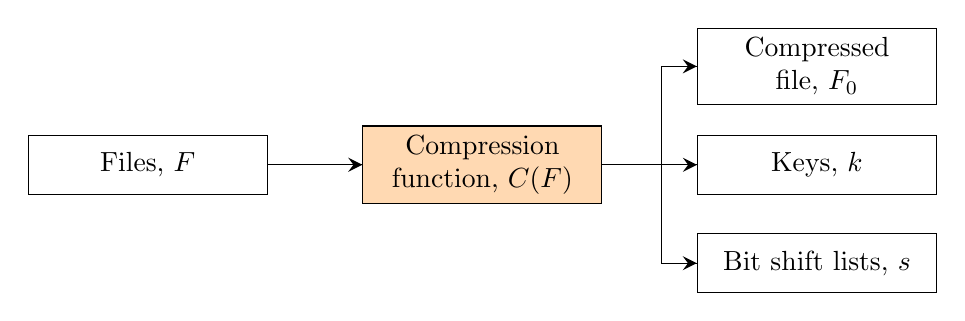
\begin{tikzpicture}[node distance=1.25cm]
        \tikzset{myptr/.style={decoration={markings,mark=at position 1 with %
    {\arrow[scale=1.6,>=stealth]{>}}},postaction={decorate}}}
        \node (encodeFunc) [function] {Compression function, $C(F)$};
        \node (fs) [basic, left of=encodeFunc, xshift=-3cm] {Files, $F$};

        \node (ks) [basic, right of=encodeFunc, xshift=3cm] {Keys, $k$};
        \node (f0) [basic, above of=ks] {Compressed file, $F_0$};
        \node (ss) [basic, below of=ks] {Bit shift lists, $s$};

        \draw [myptr] (fs.east) -- (encodeFunc.west);

        \draw [myptr] (encodeFunc.east) -| ++(0.75cm,0) |- (f0.west);
        \draw [myptr] (encodeFunc.east) -- (ks.west);
        \draw [myptr] (encodeFunc.east) -| ++(0.75cm,0) |- (ss.west);
    \end{tikzpicture}
    \caption{Visual representation of compression}
    \label{fig:encodeChart}
\end{figure}

\subsubsection{Example long key compression}\label{subsubsec:example}
Given $F_0$=\texttt{10110101} and $F_n$=\texttt{11001000}, therefore the long key must be \texttt{01111101}. However, this long key can be compressed, and represented using the key \texttt{11001} and the BSL \texttt{[0, 2]}. To expand the key and BSL pair into the long, or intermediate, key, which is XOR-ed with the master file to produce the file related with this specific BSL and key pair, the BSL is used one item at a time in the following manner once the long key has been initialised to 0. First the key is bit shifted left by the current value in the BSL. This is then XOR-ed with the long key and replaces the previously stored long key value. Using the example previously given, this would result in \texttt{11001} being first bit shifted by 0 to the left resulting in \texttt{11001}. This is then XOR-ed with the initialised long key value of 0, resulting in the long key now having a value of \texttt{11001}. The next value in the BSL is 2, so the key is bit shifted left by 2 resulting in \texttt{1100100}. This is then XOR-ed with the long key resulting in \texttt{01111101}, which is the desired long key for this $F_0$ and $F_n$.

\subsection{Expansion}\label{subsec:expansion}

\begin{figure}[ht]
    \centering
    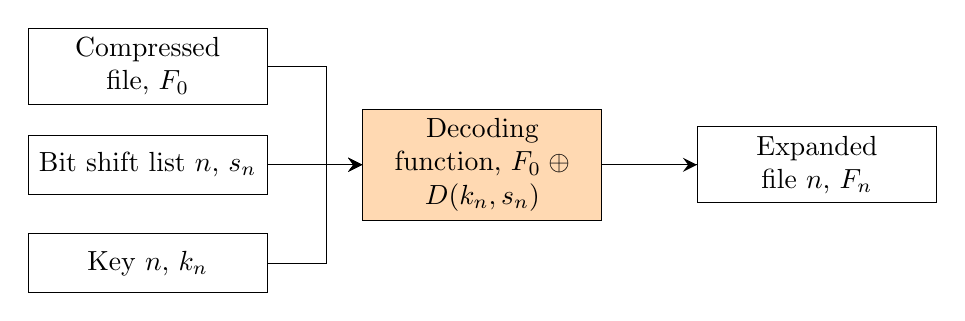
\begin{tikzpicture}[node distance=1.25cm]
        \tikzset{myptr/.style={decoration={markings,mark=at position 1 with %
    {\arrow[scale=1.6,>=stealth]{>}}},postaction={decorate}}}
        \node (decodeFunc) [function] {Decoding function, $F_0\oplus D(k_n,s_n)$};
        \node (k0) [basic, left of=decodeFunc, xshift=-3cm] {Bit shift list $n$, $s_n$};
        \node (f0) [basic, above of=k0] {Compressed file, $F_0$};
        \node (kn) [basic, below of=k0] {Key $n$, $k_n$};

        \node (fn) [basic, right of=decodeFunc, xshift=3cm] {Expanded file $n$, $F_n$};

        \draw [myptr] (f0.east) -| ++(0.75cm,0) |- (decodeFunc.west);
        \draw [myptr] (kn.east) -| ++(0.75cm,0) |- (decodeFunc.west);
        \draw [myptr] (k0.east) -- (decodeFunc.west);

        \draw [myptr] (decodeFunc.east) -- (fn.west);
    \end{tikzpicture}
    \caption{Visual representation of expansion}
    \label{fig:decodeChart}
\end{figure}

The expansion method of SBX is incredible simple, requiring only a few bit shifts left and XOR functions. To expand a file, the master file $F_0$ is XOR-ed with $D(k_n,s_n)$, resulting in $F_n$, showin in \cref{eqn:decodingAll}.

\begin{equation}\label{eqn:decodingAll}
    F_n=F_0\oplus D(k_n, s_n)
\end{equation}

\section{Evaluation}\label{sec:analysis}

To evaluate the effectiveness of this method, I will be using two methods; one including keys, and one without. This is meant to represent one of the end goals of this method, having memorable and human-usable keys, which would not have to be stored. From here on, these will be referred to as EM1, with keys, and EM2, without keys (for evaluation method 1 and 2 respectively). Both methods will be use five measures to evaluate the efficiency of this compression method. These are as follows:
\begin{itemize}
    \item $S$: A ratio of the number of batches compressed using SBX compared to the total number of batches passed in
    \item $\Delta B_s$: The average change in bits stored for the successful batch compressions
    \item $\Delta B$: The average change in bits stored for all batches regardless of whether or not the batch was considered to be compressed successfully
    \item $R_s$: A ratio of the average size of a compressed file compared to the original files for all successful compressions
    \item $R$: A ratio of the average size of a compressed file compared to the original files for all compressions regardless of success
\end{itemize}

Please note that for files with a length of approximately 16 bits or more, $\Delta B_s$ and $\Delta B$, and $R_s$ and $R$ are the same and so the value will span two columns in the results tables. Also, $\Delta B_s$ and $\Delta B$ are signed values; a negative value indicates a reduction in bits, and a positive value indicates an increase in bits.

To evaluate $S$ for EM1 and EM2, \cref{eqn:eval1} and \cref{eqn:eval2} are used respectively, where $n$ is the number of files in the batch, and $2l$ is the length of the largest input files in bits.

For all of the input files, $F$, the longest file will determine the size of all the output files. In testing this method, all files were the same size. Given that the longest input file has a size of $2l$ bits, the master file will also have a size of $2l$ bits, each key will have a size of $l + 1$ bits, and each value in each bit shift list will have a size of $\log_2l$ bits.

\begin{subequations}\label{eqn:evalMethods}
\begin{equation}\label{eqn:eval1}
    L(s) < \frac{nl-2l-n}{\log_2l}
\end{equation}
\begin{equation}\label{eqn:eval2}
    L(s) < \frac{2l(n-1)}{\log_2l}
\end{equation}
\end{subequations}

I will also be looking at the values of $L(s)$, minimum mean and maximum. This is to help evaluate the best value of $n$ for SBX to be most efficient.

\section{Results}\label{sec:results}

For each of the results tables, 1000 iterations were used. All decimals are given to five decimal places if necessary.

\begin{table}[ht]
    \centering
    \begin{tabular}{l|c c c c c|c c c c c}
        \hline
        \multirow{2}{*}{$l$ (Bits)} & \multicolumn{5}{c|}{EM1} & \multicolumn{5}{c}{EM2} \\
         & $S$ & $\Delta B_s$ & $\Delta B$ & $R_s$ & $R$ & $S$ & $\Delta B_s$ & $\Delta B$ & $R_s$ & $R$ \\
        \Xhline{3\arrayrulewidth}
        4 & 0 & N/A & 5 & N/A & 1.20833 & 1 & \multicolumn{2}{c}{-7} & \multicolumn{2}{c}{0.58333} \\
        8 & 0 & N/A & 4 & N/A & 1.08333 & 1 & \multicolumn{2}{c}{-20} & \multicolumn{2}{c}{0.52083} \\
        16 & ? & ? & ? & ? & ? & ? & ? & ? & ? & ? \\
        32 & ? & ? & ? & ? & ? & ? & ? & ? & ? & ? \\
        \hline
    \end{tabular}
    \caption{Compression results for 4, 8, and 16 bit strings for EM1 and EM2 with a batch size of 3.}
    \label{tab:resB3}
\end{table}

\begin{table}[ht]
    \centering
    \begin{tabular}{l|c c c c c|c c c c c}
        \hline
        \multirow{2}{*}{$l$ (Bits)} & \multicolumn{5}{c|}{EM1} & \multicolumn{5}{c}{EM2} \\
         & $S$ & $\Delta B_s$ & $\Delta B$ & $R_s$ & $R$ & $S$ & $\Delta B_s$ & $\Delta B$ & $R_s$ & $R$ \\
        \Xhline{3\arrayrulewidth}
        4 & 0 & N/A & 4.468 & N/A & 1.13963 & 1 & \multicolumn{2}{c}{-11.532} & \multicolumn{2}{c}{0.51462} \\
        8 & ? & ? & ? & ? & ? & ? & ? & ? & ? & ? \\
        16 & ? & ? & ? & ? & ? & ? & ? & ? & ? & ? \\
        32 & ? & ? & ? & ? & ? & ? & ? & ? & ? & ? \\
        \hline
    \end{tabular}
    \caption{Compression results for 4, 8, and 16 bit strings for EM1 and EM2 with a batch size of 4.}
    \label{tab:resB4}
\end{table}

\begin{table}[ht]
    \centering
    \begin{tabular}{l|c c c c c|c c c c c}
        \hline
        \multirow{2}{*}{$l$ (Bits)} & \multicolumn{5}{c|}{EM1} & \multicolumn{5}{c}{EM2} \\
         & $S$ & $\Delta B_s$ & $\Delta B$ & $R_s$ & $R$ & $S$ & $\Delta B_s$ & $\Delta B$ & $R_s$ & $R$ \\
        \Xhline{3\arrayrulewidth}
        4 & 0 & N/A & 4.584 & N/A & 1.1146 & 0.999 & -15.43243 & -15.416 & 0.48919 & 0.4896 \\
        8 & ? & ? & ? & ? & ? & ? & ? & ? & ? & ? \\
        16 & ? & ? & ? & ? & ? & ? & ? & ? & ? & ? \\
        32 & ? & ? & ? & ? & ? & ? & ? & ? & ? & ? \\
        \hline
    \end{tabular}
    \caption{Compression results for 4, 8, and 16 bit strings for EM1 and EM2 with a batch size of 5.}
    \label{tab:resB5}
\end{table}

\begin{table}[ht]
    \centering
    \begin{tabular}{l|c c c c c|c c c c c}
        \hline
        \multirow{2}{*}{$l$ (Bits)} & \multicolumn{5}{c|}{EM1} & \multicolumn{5}{c}{EM2} \\
         & $S$ & $\Delta B_s$ & $\Delta B$ & $R_s$ & $R$ & $S$ & $\Delta B_s$ & $\Delta B$ & $R_s$ & $R$ \\
        \Xhline{3\arrayrulewidth}
        4 & 0 & N/A & 5.692 & N/A & 1.11858 & 0.99 & -18.51313 & -18.308 & 0.48931 & 0.49358 \\
        8 & ? & ? & ? & ? & ? & ? & ? & ? & ? & ? \\
        16 & ? & ? & ? & ? & ? & ? & ? & ? & ? & ? \\
        32 & ? & ? & ? & ? & ? & ? & ? & ? & ? & ? \\
        \hline
    \end{tabular}
    \caption{Compression results for 4, 8, and 16 bit strings for EM1 and EM2 with a batch size of 6.}
    \label{tab:resB6}
\end{table}

\begin{table}[ht]
    \centering
    \begin{tabular}{l l|c c c}
    \hline
        \multirow{2}{*}{$n$} & \multirow{2}{*}{$l$ (Bits)} & \multicolumn{3}{c}{$L(s)$ data} \\
         & & Min. & Mean & Max.\\
        \Xhline{3\arrayrulewidth}
        \multirow{4}{*}{3} & 4 & 3 & 3 & 3 \\
         & 8 & 3 & 3 & 3 \\
         & 16 & ? & ? & ? \\
         & 32 & ? & ? & ? \\
        \hline
        \multirow{4}{*}{4} & 4 & 4 & 4.224 & 5 \\
         & 8 & ? & ? & ? \\
         & 16 & ? & ? & ? \\
         & 32 & ? & ? & ? \\
        \hline
        \multirow{4}{*}{5} & 4 & 5 & 5.792 & 14 \\
         & 8 & ? & ? & ? \\
         & 16 & ? & ? & ? \\
         & 32 & ? & ? & ? \\
        \hline
        \multirow{4}{*}{6} & 4 & 6 & 7.846 & 28 \\
         & 8 & ? & ? & ? \\
         & 16 & ? & ? & ? \\
         & 32 & ? & ? & ? \\
        \hline
    \end{tabular}
    \caption{Caption}
    \label{tab:L(s)Analysis}
\end{table}

\begin{acknowledgements}
The research presented in this paper was aided in part by the MPI library for python, \cite{DALCIN20051108}. I would also like to thank Rosetta Code for their code published on finding the first non-zero bit in a binary string \cite{rosetta_code_2021}.
\end{acknowledgements}

\printbibliography

\end{document}
